\section{Itthipaṇḍaka, Animittā, Nimittamattā, Vepurisikā}

These four terms mentioned in the {\em Bhikkhunikkhandhaka} are rather vague in their descriptions\footnote{See \ref{appendix1} for a detailed listing of the the occurances of the words in the Buddhist canon in Pāli and Chinese together with some of the existing interpretations and translations.}. The Chinese texts are not very clear on this point either but the overall questions asked here seem to have mostly to do with menstruation and diseases. At first glance it seems that the rules regarding ordination are trying to make sure that the girl in question is old enough for ordination and not ill. Rules concerning whether or not a girl has breasts can be explained as a question with regards to age, or it can be explained as a girl who has not developed the secondary characteristics needed i.e. possibly intersex. We will never know the true purpose behind these questions but it is not unlikely that these questions about the development of sexual organs were asked for the sole purpose of establishing age. After all, we also find rules in the {\em Bhikkhunīpātimokkha} that prohibit the ordination of married girls under the age of 12\footnote{{\em Pācittiya 65 Yā pana bhikkhunī ūnad­vāda­sa­vassaṃ gihigataṃ vuṭṭhāpeyya, pācittiyaṃ.}}. The question about whether a girl is sterile or barren would point to her at least having had one child (how else would they know if she is fertile) but this would seem strange if she wants to enter a celibate order. It might be a question meant to find out if she is at least menstruating. 

Bhikkhu Sujato points out that the Bhikkhunī Vinaya uses its own language and terminology that is often more in line with the Jain terminology and is poorly integrated with the Bhikkhu Vinaya\footnote{\cite{sujato2009} page 143–145}. This could explain the discrepancies we see between the Bhikkhu and Bhikkhunī Vinaya in describing certain words pertaining to gender. In any case, the variabilty and vagueness of these terms with reference to gender do not permit a clear picture.

The following table gives an overview of the terms:

\bigskip
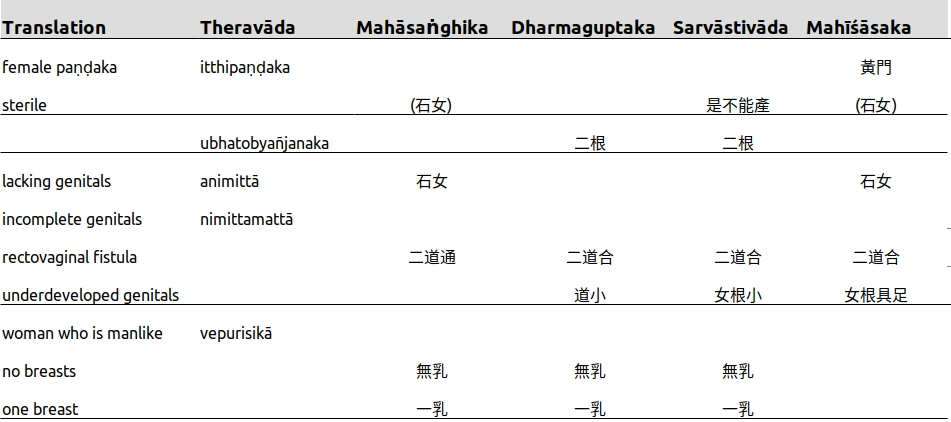
\includegraphics[width=\linewidth]{female.jpg}
\label{female}

It is certain though that the terms of {\em paṇḍaka} and {\em ubhatob­yañ­janaka} pertained primarily to male candidates as we have also seen in the Jain order while the Bhikkhunī seem to have had their own vocabulary.

There are some rare cases of people who are raised from birth as girls that later became assigned as hijra after they failed to develop secondary female sexual characteristics (breast development and menarche) at puberty\footnote{\cite{nanda} page 15}. Although there is very little evidence to go on, I believe that these could possibly be representing the {\em itthipaṇḍaka}. The {\em itthipaṇḍaka} does not appear in any but the Pali scriptures while the Chinese talk about a 'barren/sterile woman', which could be the same or not. Only the Mahīśāsaka Vinaya talks about a 黃門.

At least in the Bhikkhunī ordination in the Theravāda lineage, the {\em animittā, nimittamattā and vepurisikā} are allowed to ordain. This is possibly also true in several of the Chinese Vinaya.

\section{Changing Gender}

The Theravāda Vinaya {\em Bhikkhu Pā­rāji­ka} 1 lists the curious case where a monk changes characteristics and is now seen as a woman. She is then admitted into the Bhikkhunī order. The same holds true for a nun who changes sex/gender and is from that moment on a Bhikkhu.

The same passage is found in several of the Chinese schools\footnote{This passage possibly appears in all of the Chinese schools but I have been unable to locate it} below the passages on ordination. Again the Chinese words are confusing here, mixing up the words for 'root' and 'shape', which seem to be used as synonyms.

The Buddha seems to handle this rather curious matter (after all, it does not seem to be likely that anybody just changes gender from one day to the next) in a very matter-of-fact way. The monastic in question is simply assigned in the other order while keeping their years of seniority. It does not seem to be a problem at all.

What is interesting here is the words for 'characteristic' used. In the Chinese 根 ('root', quite often glossed as meaning 'genitals') or 形 ('shape/form') is use, the Theravāda text uses {\em liṅga}. As we have seen in the chapter on the historical development of the terms in the Brahmanical and Jain context, the original meaning of {\em liṅga} is 'characteristic mark or sign' and only later became to mean 'sexual characteristics'; it caused much confusion and debate. Around the time of the Buddha, the term did not have a very definate meaning, also including characteristics like long hair (as female) and according to the Jain it could be a combination of sex, behavior, physical characteristics and also the underlying sexuality and feelings. 

In the absense of modern inventions like Hormone Replacement Therapy or surgery, it seems unlikely that somebody would completely change sex overnight. 




--------------------------------------------------------------------


Still to do:


Claire's
BS Vinaya studies







Religion plays a large role in socializing individuals to their assigned gender-roles. Buddhism is certainly no exception to that, but we have to make a difference here between the Buddha’s teachings, and Buddhist culture, which has developed based on geographical and interpretational differences since the time of the Buddha.

In order to understand the Buddhist’ point of view we have to go back in history. As Ayya Sujato pointed out in his article on the Buddha’s genitals 16, the Buddhas himself appears to be more non-binary: he has gone beyond the notion of gender. But how were things in the Buddha’s time? This was a very different society than ours and the only things we know about it have come to us through the background stories of the Suttas and the Vinaya. But what that tells us is that in social relationships, this society was not so very different from India today. In any case, it was most likely a hetero-patriarchical society where forced marriage was the norm.

It was in this society that the Buddha had to teach. Even if he himself felt different, he would not directly challenge existing structures in society but would teach people to contemplate and look inside of themselves. His way of teaching was very subtle, never lecturing but always guiding people to find answers inside. And what he taught was to be compassionate to all beings, regardless of caste and gender.

In his Teachings he makes very clear that these distinctions between humans are irrelevant:

“Neither in neck, nor shoulders found,
not in belly or the back,
neither in buttocks nor the breast,
not in groin or sexual parts.

Neither in hands nor in the feet,
not in fingers or the nails,
neither in knees nor in the thighs,
not in their “colour”, not in sound,
here is no distinctive mark
as in the many other sorts of birth.

In human bodies as they are,
such differences cannot be found:
the only human differences
are those in names alone.”

Suttanipāta 3.9 4

The Teachings
There are various ways to look at the teachings. One way which I find very helpful here is the teachings on the five Khandhas: form, feeling, perception, choices and consciousness. When teaching about the five Khandhas, the Buddha teaches to contemplate them as Anicca (impermanence), Dukkha (suffering) and Anatta (not-self). He does not say that there is not a self, but that if you identify with a self, you actually identify with these five Khandhas; if you see them in accordance with reality, they don’t operate as a “self”, something you can cling to.

His approach is to encourage investigation. How do you know these things? Go through each aspect of experience and see if it is permanent of impermanent. “Dukkha” is a bit more subtle and sometimes confusing because the term “dukkha” is here used as a characteristic of the five Khandhas and is not used in the same sense as the feeling of “dukkha”, which is part of the second Khandha. What is meant here is something like seeing the imperfection of things, seeing that it is not fit to provide lasting satisfaction. Anatta is seeing that these experiences cannot be controlled and are therefore not a self.

One of the most important things about the five Khandhas is not the particular definition of each each but the interrelationship between the first four (form, feeling, perception, choices) with the fifth (consciousness). The interaction, the responsiveness and the resonance between the inner subjective awareness and the sentient body, between the inner sense of awareness and the external signs. We don’t simply see objects as annica, dukkha, Anatta but the very nature and structure of the interaction itself is interdependent and constantly spinning around, constantly changing. Deep insight is not about knowing what external objects are but how the mind is involved with these objects.

In relation to gender, we can see that our gender-identity is a perception. Whether we identify as man, woman or something else, we all have this perception. We also have an idea about how other people perceive us and this is where our assigned gender-role comes into play. This gender-role is a socially conditioned phenemenon, but it also has an internal part, namely how we perceive this in relation to ourselves; the interaction between what is inside and what is outside. We have no control over how these things are and we cannot will ourselves to have a different gender-identity. It is Anatta. It is as it is and we cannot change it. Our gender-identity is not a choice.

But when contemplating, there is a shift from Sañña (perception) to Pañña (wisdom). By observing things, slowly our defilements disappear and we will start to see things in a different light. The inner qualities of the mind change while wisdom grows. This way, we can let go of our thinking about how we “should be” according to some perceived social standard outside of us and learn to accept ourselves, and our gender, as we are, while keeping in mind that it is Anatta. This way we change our relationship to the outside world and we change our perception of ourselves and others.

The Vinaya
As is shown in the short video 6 that @Adan posted, the argument against transgenders ordaining that is used now is the same as was used for Bhikkhunis before: you can meditate and develop without being ordained, just accept the way it is and be content with that. This is an argument that is used often by Buddhists, therewith quoting the Teachings of being content, equanimous and letting go. But that is a wrong grasp of the Teachings. Wanting to ordain is a wholesome aspiration and in line with the Dhamma and the Buddha would have applauded that. The Buddha himself was always compassionate to all beings and when individuals were refused ordination it was never because of their gender-identity or sexual orientation.

We have to look at how people with another gender were described in the Vinaya. There are several words that could denote this, or are generally translated as such, all of which only appear in the Khandakas of the Vinaya Pitaka and more precisely only in the Bhikkhunikhandaka (or as a term of abuse in Bhikkhu Saṅghādisesa 3 1). Bhikkhu @Sujato (2007) argues that the Bhikkhunikkhandhaka, as well as other parts of the Vinaya, are a later addition, possibly dating back to the Second Council.

There are several types of people that are noted: Vepurisikā, Sambhinna, Ubhatovyañjanaka and Paṇḍaka.
All of these terms are mentioned in conjunction with ordination: people with these characteristics are not allowed to ordain, at least, not as a Bhikkhuni. In the Early Buddhist Suttas we do not find any mention of the first three terms, only the word Paṇḍaka is found in some Anguttara Nikaya passages that do not have any parallels in other Early texts. It is not well understood what these terms actually denote, although the more conservative people in the Sangha refer to these terms as meaning anybody who does not comply with the established gender-norms. However, I believe it is wrong to accept the most conservative reading of the texts based on so little knowledge of the actual meaning of these terms.

The term Paṇḍaka has been discussed in more detail in this thread 4 and also in the essay by @Bernat Font 1. It would seem that a Paṇḍaka is not an indication of gender or sexual orientation but more a term denoting a person who exhibits strong lustful behavior that would of course be inappropriate in the Sangha.

Regardless of how the Vinaya is interpreted, the doctrine of Anatta itself denies that there is an identity or lasting entity at the centre of any being, so this makes gender difference at the deepest level a superficial factor just as race, ethnicity, appearance or social status. Therefore to deny anybody ordination on the basis of this is itself against the Dhamma.

The Buddha’s teachings are just as applicable in today’s world as they were 2500 years ago, but we have to keep in mind that the conditions in which we need to work with these teachings are vastly different. We have no Buddha to tell us what to do, but if we try to follow the Buddha’s footsteps and be kind and compassionate to all beings, we cannot be far off.

Bhikkhu or Bhikkhunī?
Of course the above begs the question: if ordination for transgenders is allowed … how should they ordain?

No doubt this will be the topic of much discussion in years to come because not all trans-people also have had surgery (so they might still have the body of the opposite sex, at least partly). It is quite possible that somebody with male genitals identifies as a woman and visa versa. Moreover, there are many people who don’t strongly identify with either sex: they are non-binary.

Anderson (2016a) points out that monks and nuns forego the usual markers of sex and gender difference when they don their robes and shave their heads. In addition to this, they live a celibate life so these sexual organs are not used for the purpose that nature designed them for. It would therefore seem ludicrous for a transgender, who has not had full surgery, to have to go through this for the sake of a body part that plays no part in Buddhist Monastic practice.

The argument revolves around the explanation of a passage in the Vinaya in Pārājika 1 (translation by Ajahn @Brahmali):

At one time the characteristics of a woman appeared on a monk. They informed the Master. He said: “Monks, I allow that very discipleship, that very ordination, those years as a monk, to be transferred to the nuns. The monks’ offenses that are in common with the nuns are to be dealt with in the presence of the nuns. For the monks’ offenses that are not in common with the nuns, there’s no offense.”

The same passage is then repeated for a nun.

The appearance of this passage in Pārājika 1 is a bit odd. This rule has to do with sexual intercourse and obviously a change of characteristics has nothing much to do with that. It is possible that this passage was added later.

Carol Anderson (2016) points out that in the Abhidhamma, male rebirth is seen as the result of good kamma and female rebirth as the result of bad kamma (adultry) and that this might have some bearing on the appearance of this passage in Pārājika 1.

It is unclear what exactly “characteristics of a (wo)man” are. The word this hinges on is liṅga, which means sign or characteristics. It can refer to physical characteristics but not necessarily. The words for “characteristics of a (wo)man” are itthiliṅgaṃ and purisaliṅgaṃ. These words appear in the canon only 5 times, in later texts like the Abhidhamma and the Milindapañha. It also appears in the early suttas once, namely in Digha Nikāya 27 which describes the evolution. In the latter case, it seems that liṅga indeed refers to biological sex.

In the first commentary on the Vinaya-piṭaka, the Samantapāsādikā, the change of liṅga is described as appearing suddenly in the middle of the night; one goes to bed as a man and wakes up as a woman. This seems of course highly unlikely but might have it’s roots in the notion that sleep is a precarious state whereby one looses control, which can lead to shameful situations (Heirman, 2012). The commentary also attributes such a change to good or bad kamma.

Scherer (2006) and others take the term liṅga as a reference to the ‘secondary sex organs’ or characteristics of sexual difference, which also include behavioral differences so the term can be used to denote both biological sex and gender-identity as we define it today. They base this conclusion on the work of Buddhaghosa, a later commentator. However, the notion of gender as we have today is no doubt different from that in the time of the Buddha. More research in this field and also the corresponding parallels in other schools is needed to get a better picture.

In any case, it seems that there is a lot of uncertainty about what liṅga actually refers to. There are different attempts to explain the term in later commentarial literature but these have very different views from each other. All this has an impact on the ordination procedure, whereby one is asked if one is a purisa(man) or itthi (woman). It would follow from this passsage in Pārājika 1 that in order to be a man or woman for the purpose of ordination, one should have the liṅga of a man or woman.

I feel that the safest way to approach this is again to look at the Teachings and choose the most compassionate route. The passage in Pārājika 1 gives an indication of what the Buddha would do: the transitioned person should practice according to the VInaya that is most appropriate to them in order to get the best possible opportunities to eradicate defilements and practice the teachings.

I feel therefore that in light of the Teachings, ordination should be based on gender-identity and not on biological sex. The Buddha’s Vinaya is a guideline for our practice and is meant to help us overcome our defilements. A trans-woman, because of her gender-identity as a woman, will also benefit more from the training for Bhikkhunis and visa versa. It is therefore up to each individual to see where they would receive the best training suited for them in consultation with the monastics of the monastery where they wish to train.

As Ajahn Brahm said:

As Buddhists who espouse the ideal of unconditional loving kindness and respect, judging people on their behavior instead of their birth, we should be well positioned to show leadership on the development of gender equality in the modern world and the consequent reduction of suffering for half the world’s population. Moreover, if Buddhism is to remain relevant and grow, we must address these issues head on. But how can we speak about gender equality when some of our own Theravada Buddhist organizations are gender biased?

In this article I do not aim to be complete but try to create an overview of the issues and open a channel for discussion and more research in this field. Now we have some fairly comprehensive research with regards to Bhikkhunis and the possibility of Bhikkhuni ordination, it is time we start to look at other minorities that are not always accepted within the Sangha.

References:
Anderson, C. (2016). Changing Sex in Pali Buddhist Monastic Literature. Researchgate.
https://www.researchgate.net/publication/313629904_Changing_Sex_in_Pali_Buddhist_Monastic_Literature 3

Anderson, C. (2016a). ‘Defining Women’s Bodies in Indian Buddhist Literature’ In: Barbara A. Holdrege and Karen Pechilis (eds) Re-figuring the Body: Embodiment in South Asian Religions. Albany, NY: State University of New York Press

Begley, S. (2009, June 29). Don’t blame the caveman. Newsweek 52–62.

Buller, D. J. (2006). Adapting minds: Evolutionary psychology and the persistent quest for human nature. Cambridge, MA: MIT Press.

Heirman, Ann 2012. ‘Sleep Well! Sleeping Practices in Buddhist Disciplinary Rules’ Acta Orientalia Academiae Scientiarum Hungaricae 65(4), pp. 427–444.

Hurley, S. (2007). Sex and the social construction of gender: Can feminism and evolutionary psychology be reconciled? In J. Browne (Ed.), The future of gender (pp. 98–115). New York, NY: Cambridge University Press.

Lindsey, L. L. (2011). Gender roles: A sociological perspective (5th ed.). Upper Saddle River, NJ: Prentice Hall.

Mead, M. (1935). Sex and temperament in three primitive societies. New York, NY: William Morrow.

Morgan, S. (Ed.). (1989). Gender and anthropology: Critical reviews for research and teaching. Washington, DC: American Anthropological Association.

Murdock, G. (1937). Comparative data on the division of labor by sex. Social Forces, 15, 551–553.

Salt D, Brain Z (June 2007). “Intersex: Case studies”. Cosmos (15). Archived from the original on 2009-02-14.

Scherer, Burkhard (2006). ‘Gender Transformed and Meta-gendered Enlightenment: Reading Buddhist Narratives as Paradigms of Inclusiveness’ Revista de Estudos da Religião – REVER 6(3), pp. 65–76.

Sirimanne, Chand R. (2016). Buddhism and Women-The Dhamma Has No Gender. Journal of International Women’s Studies.
http://vc.bridgew.edu/cgi/viewcontent.cgi?article=1923&context=jiws 1


